\chapter{Evaluation}
\label{cha:evaluation}
\section{Experiment Environment}
\subsection{Compiler}
\label{section:compiler}
Minizinc IDE~\footnote{\url{https://www.minizinc.org/}}, developed by the University of Melbourne, Monash University and Data61 Decision Sciences, is a compiler which allows users to edit and run their models~\cite{r6}. It provides some built-in functions as well as optimization methods. In our models, the build-in algorithm that aims to achieve singleton arc consistent and the built-in Minizinc-to-Flatzinc translator have been applied. In addition, a wide range of solvers has been tested~\cite{r6}. In our case, because the CSPs can be considered as mixed-integer programming (MIP) problems too, some MIP solvers are used to evaluate.
\begin{itemize}
    \item \emph{Choco}: A Java CSP solver, which supports many search strategies (DomWDeg, ABS, IBS, first-fail, etc.) and optimization processes (LNS, fast restart).
    \item \emph{Chuffed}: A C++ finite domain solver using lazy clause generation, which contains a nogood logbook to avoid plenty of duplicate calculations.
    \item \emph{Coin-bc}: A C++ based MIP solver, it adopts the branch and cut optimization.
    \item \emph{Gurobi}: A commercial solver supports MIP.
    \item \emph{Izplus}: Based on iZ-C constraint programming that is developed by NTT DATA SEKISUI SYSTEMS CORPORATION. It combines Randomized restarting, Local search, Variable reordering and nogood learning.
    \item \emph{Jacop}: A Java CSP solver.
    \item \emph{OR-Tools}: An open-source solver developed by google, it combines many optimization methods.
    \item \emph{PicatSAT}: A CSP solver based on picat which is a rule-based language. And it adopts log encoding~\cite{r8}.
    \item \emph{Yuck}: Based on Scala and combines local search with restarting, global constraints, and lexicographic cost functions.
\end{itemize}
\subsection{Software Platform and Hardware Platform}
\label{sec:softplat}
Most of the experiments are based on the Windows subsystem for Linux 2 (WSL2)~\footnote{\url{https://docs.microsoft.com/en-us/windows/wsl/about}} which allows the developer to run a Linux environment on Windows 10. Only the experiments related to izplus based on docker. Docker is a lightweight virtual machine that applied container virtualization technology~\cite{r25}. Docker provides a Linux environment as well. Table~\ref{tab:Ubuntu} shows the version of WSL2.
\begin{table*}[htbp]
  \centering

  \caption{The version of Windows subsystem for Linux 2}
  
  \label{tab:Ubuntu}
  \input table/Ubuntuversion.tex
\end{table*}
Furthermore, as mentioned in Chapter~\ref{section:compiler}, there are nine solvers that have been applied in our experiment, Table~\ref{tab:solvers} indicates the version of each solver.
\begin{table}[htbp]
  \centering

  \caption{The deployed solvers and corresponding versions}
  
  \label{tab:solvers}
  	\begin{subtable}[b]{\textwidth}
  	\centering
  \input table/solver1.tex
    \end{subtable}\\
    	\begin{subtable}[b]{\textwidth}
  	\centering
  \input table/solver2.tex
  \end{subtable}\\
  \begin{subtable}[b]{\textwidth}
  \centering
  \input table/solver3.tex
  \end{subtable}
\end{table}
\\In addition, Table~\ref{tab:machines} introduces the configurations of the hardware platform.
\begin{table}[H]
  \centering

  \caption{Processor used in our evaluation}
  
  \label{tab:machines}
  \input table/machines.tex
\end{table}
Moreover, based on the experiment environment, all experiment results and corresponding codes are available at~\footnote{\url{https://gitlab.cecs.anu.edu.au/u1092535/project-2020-s2-puzzle-constraints}}.
\section{Results}
\label{sec:Result}
In this section, both the results of IQ Twist's experiments and the results of Zig Zag Puzzler's experiments will be discussed. Generally, all the problems in both games' booklets have been tested by the nine solvers that are mentioned in Table~\ref{tab:solvers}. For each game, there are five difficulties 'start', 'junior', 'expert', 'master' and 'wizard'. Each difficulty consists of some problems. The time limit for running each problem is 30 minutes, which is represented as 1800 seconds. If the solver can get the result in 1800 seconds, the time will be logged, otherwise, it will be treated as an unsolved problem, and the execution time will be logged as 1800 seconds. 
\\Above all, the discussions for the result will mainly include two parts, the coverage rate and the execution time of each solver. 
\\For the coverage rate, it can be calculated by 
\begin{equation}
\label{equation:coverage}
   C= N1/N2,
\end{equation}
where $C$ means the coverage rate, $N1$ means the number of solved problems and $N2$ means the number of total problems, in our case, the overall coverage rate and separated coverage rates that correspond to different difficulties will be discussed.
\\And for the execution time, except for all execution time, the average execution time will be considered as well. It can be calculated by 
\begin{equation}
\label{equation:averagetime}
\overline{t}=\frac{\sum\limits_{i=1}^n t_{i}}{n},
\end{equation}
where $\overline{t}$ is the average execution time, $\sum\limits_{i=1}^n t_{i}$ is the sum of execution time for each problem and $n$ is the number of problems.
\subsection{IQ Twist Results}
\label{sec:IQtwistresults}
In the IQ twist booklet, there is a total of 120 problems with 5 difficulties, every 24 problems make up a difficulty. 
\begin{table}[htbp]
\centering
\caption{Overall solved problems for each solver (a total of 120 problems)}
\label{tab:solvedproblem}
\begin{tabular}{|l|l|l|l|l|l|l|l|l|}
\hline
Choco & Chuffed & Coinbc& Gurobi & Izplus&Jacop& OR-Tools& PicatSAT&Yuck \\
\hline
119   &120      & 4     & 108    &84     &58   &120    &120      &36\\
\hline
\end{tabular}
\end{table}
\\Firstly, for each solver, we can calculate the overall coverage rate by Equation~\ref{equation:coverage}.
\begin{figure}[H]
     \centering
    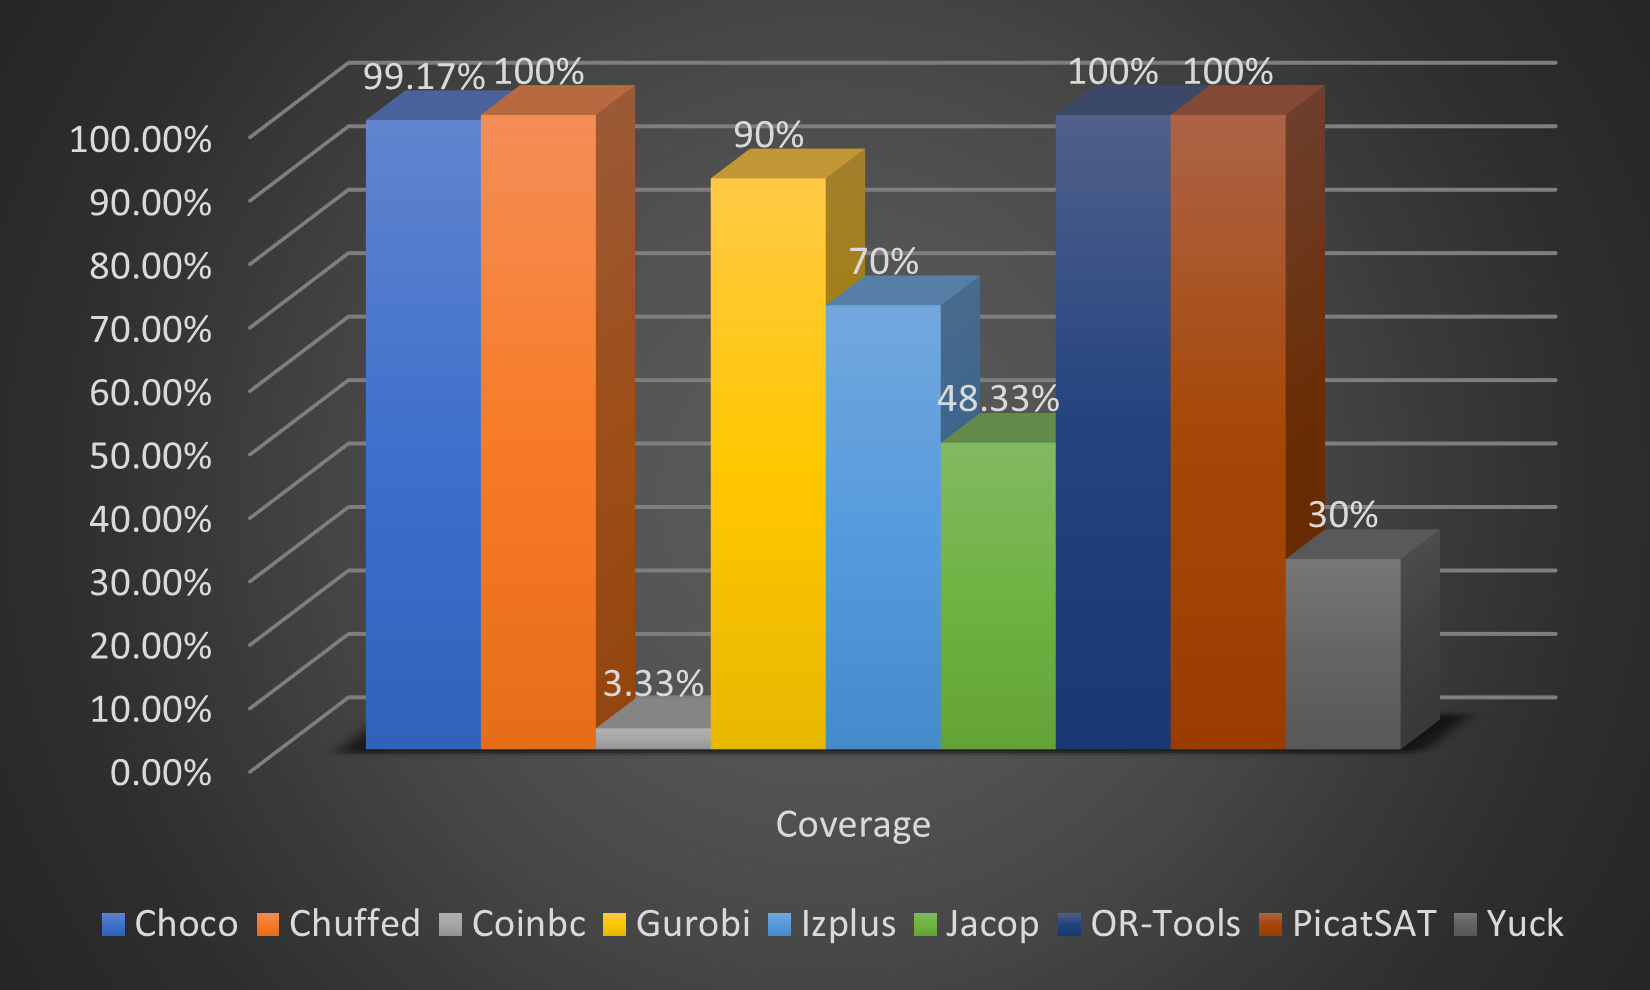
\includegraphics[width=0.8\textwidth]{figs/coverage.png}
    \caption{Overall coverage rate of each solver}
    \label{eva2}
\end{figure}
Table~\ref{tab:solvedproblem} shows the solved problems for each solver. Based on the data in Table~\ref{tab:solvedproblem},
Figure~\ref{eva2} shows the overall coverage rates for different solvers, which indicates that there are only 3 solvers with an overall coverage rate of 100 percent.
In addition, Table~\ref{tab:solvedproblemforeach difficulty} separately shows the solved problems of different difficulties for each solver. 
\begin{table}[htbp]
\centering
\caption{Solved problems of each difficulty (a total of 24 problems for each difficulty)}
\label{tab:solvedproblemforeach difficulty}
\begin{tabular}{|l|l|l|l|l|l|}
\hline
	    &Start&	Junior&	Expert&	Master&	Wizard\\
\hline
Choco   &23   &24 &24 &24 &24\\
\hline
Chuffed	&24   &24 &24 &24 &24\\
\hline
Coinbc	&4    &0  &0  &	0 &0\\
\hline
Gurobi	&24   &22 &20 &	23&19\\
\hline
Izplus	&23   &21 &13 &	17&10\\
\hline
Jacop	&20   &9  &11 &13 &5\\
\hline
OR-Tools	&24   &24 &24 &	24&24\\
\hline
PicatSAT&24   &24 &24 &24 &24\\
\hline
Yuck    &13	  &6  &2  &7  &8\\
\hline
\end{tabular}
\end{table}
Accordingly, Figure~\ref{fig:comparisonIQtwist} illustrates the change of separated coverage rates as the increase of difficulties. It seems like the separated coverage rates of other solvers are not stable in different difficulties except there are 3 solvers which always keep 100 percent. In other words, there is no obvious relationship between the separated coverage rates and difficulties. Because the method to set the difficulty of IQ Twist is a change of the pegs' positions, and the number of placed pegs has no relationship with difficulties, the change of the number of search nodes is tiny. 
\begin{figure}[H]
    \centering
    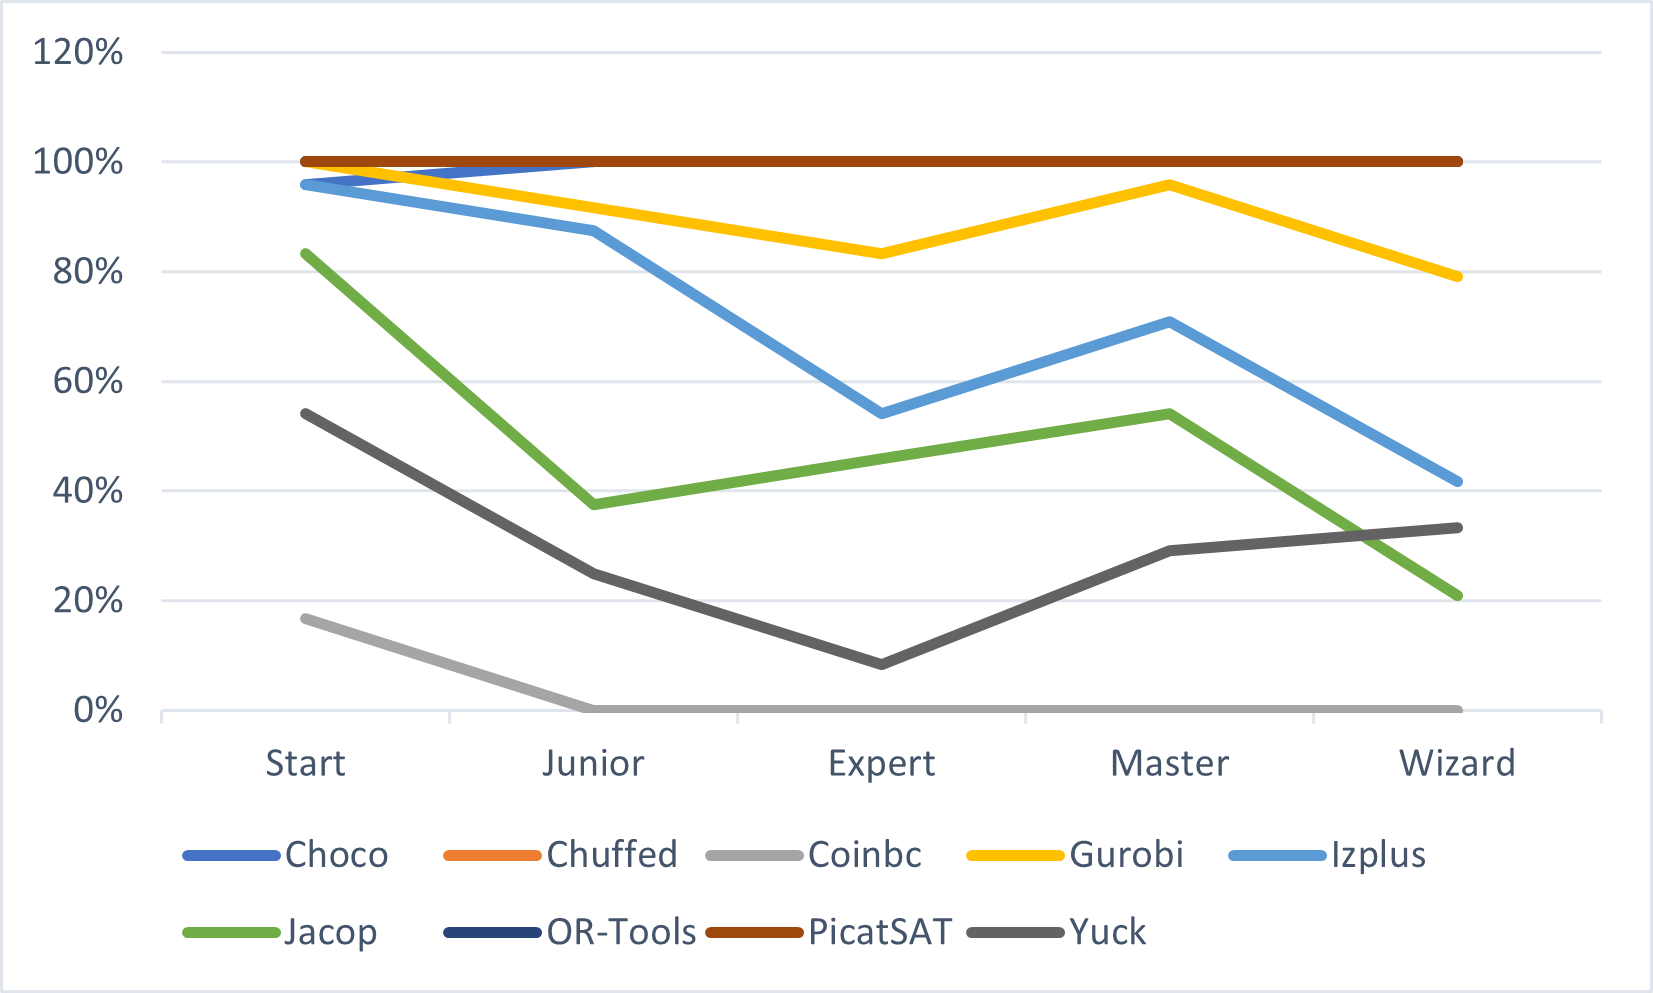
\includegraphics[width=0.8\textwidth]{figs/separated coverage.png}
    \caption{Coverage rates of each difficulty}
    \label{fig:comparisonIQtwist}
\end{figure}
Therefore, compared with other solvers, PicatSAT, OR-Tools and Chuffed take an advantage in coverage rates.
\\Secondly, all the execution time have been shown in Figure~\ref{fig:execution time}.
\begin{figure}[H]
    \centering
    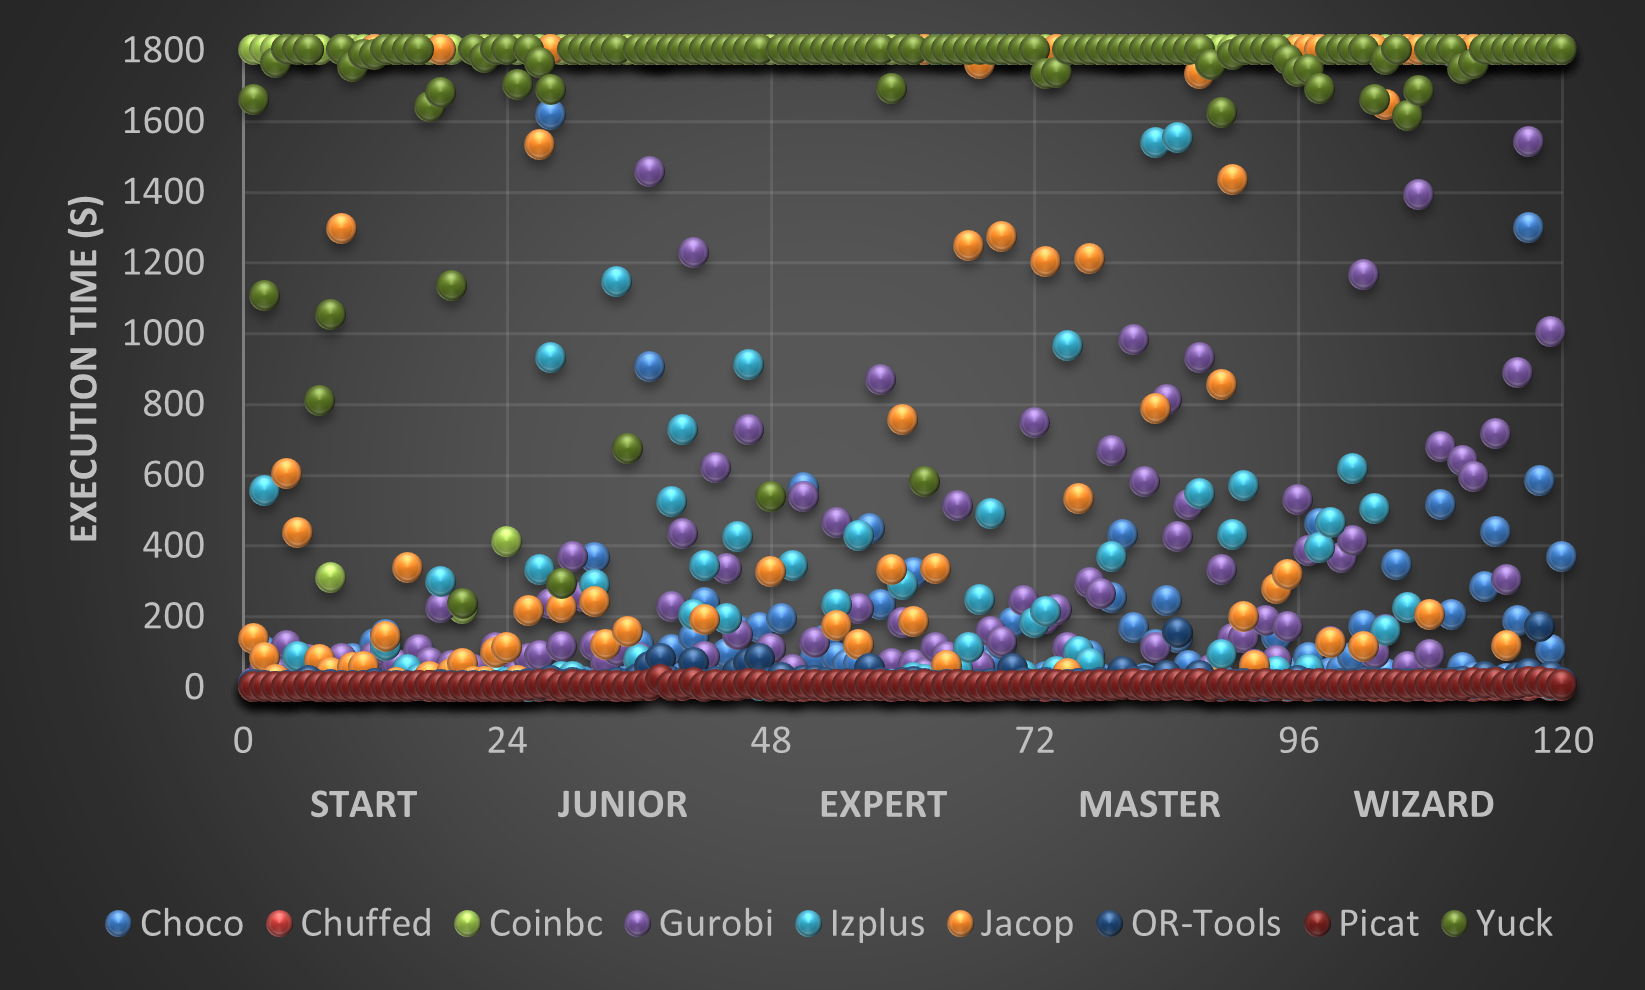
\includegraphics[width=0.8\textwidth]{figs/all_point_IQtwist.png}
    \caption{All execution time of all solvers}
    \label{fig:execution time}
\end{figure}
Figure~\ref{fig:execution time} indicates that Chuffed, PicatSAT and OR-Tools take huge advantages compared with other solvers because the three solvers can solve each problem in only 200 seconds.
\begin{figure}[H]
\centering
\begin{subfigure}[b]{.48\textwidth}
\centering
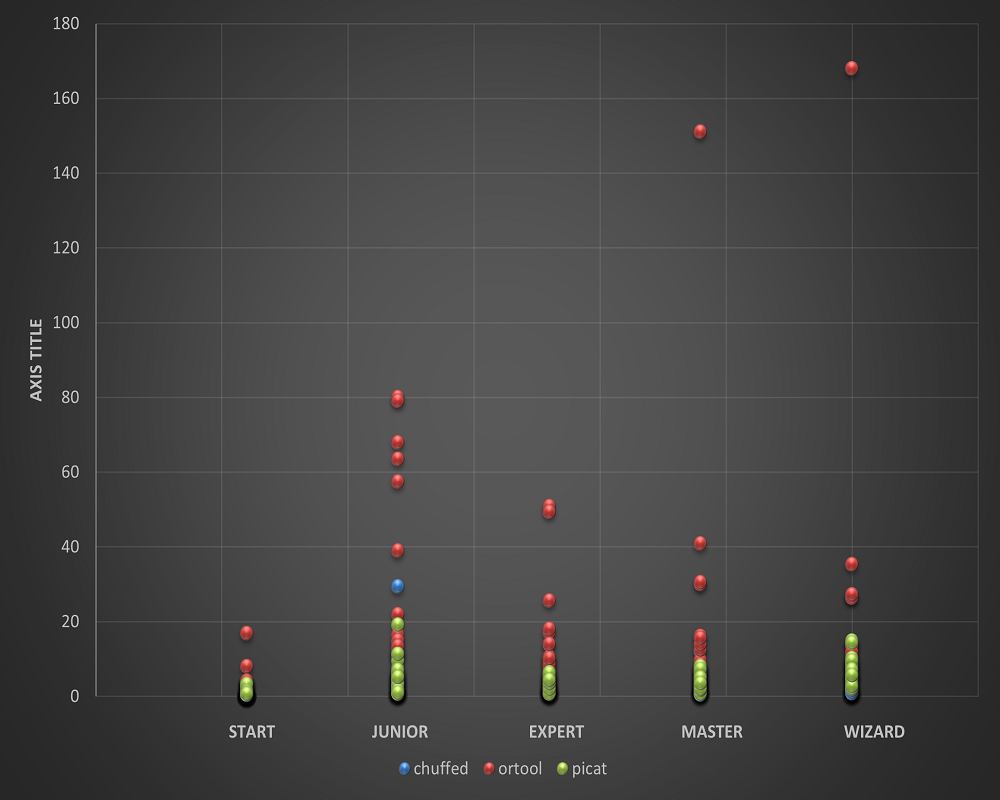
\includegraphics[width=\textwidth]{figs/threesolverpoints.png}
\caption{Execution time for Chuffed, PicatSAT and OR-Tools}
\label{fig:3solvers1}
\end{subfigure}
\begin{subfigure}[b]{.48\textwidth}
\centering
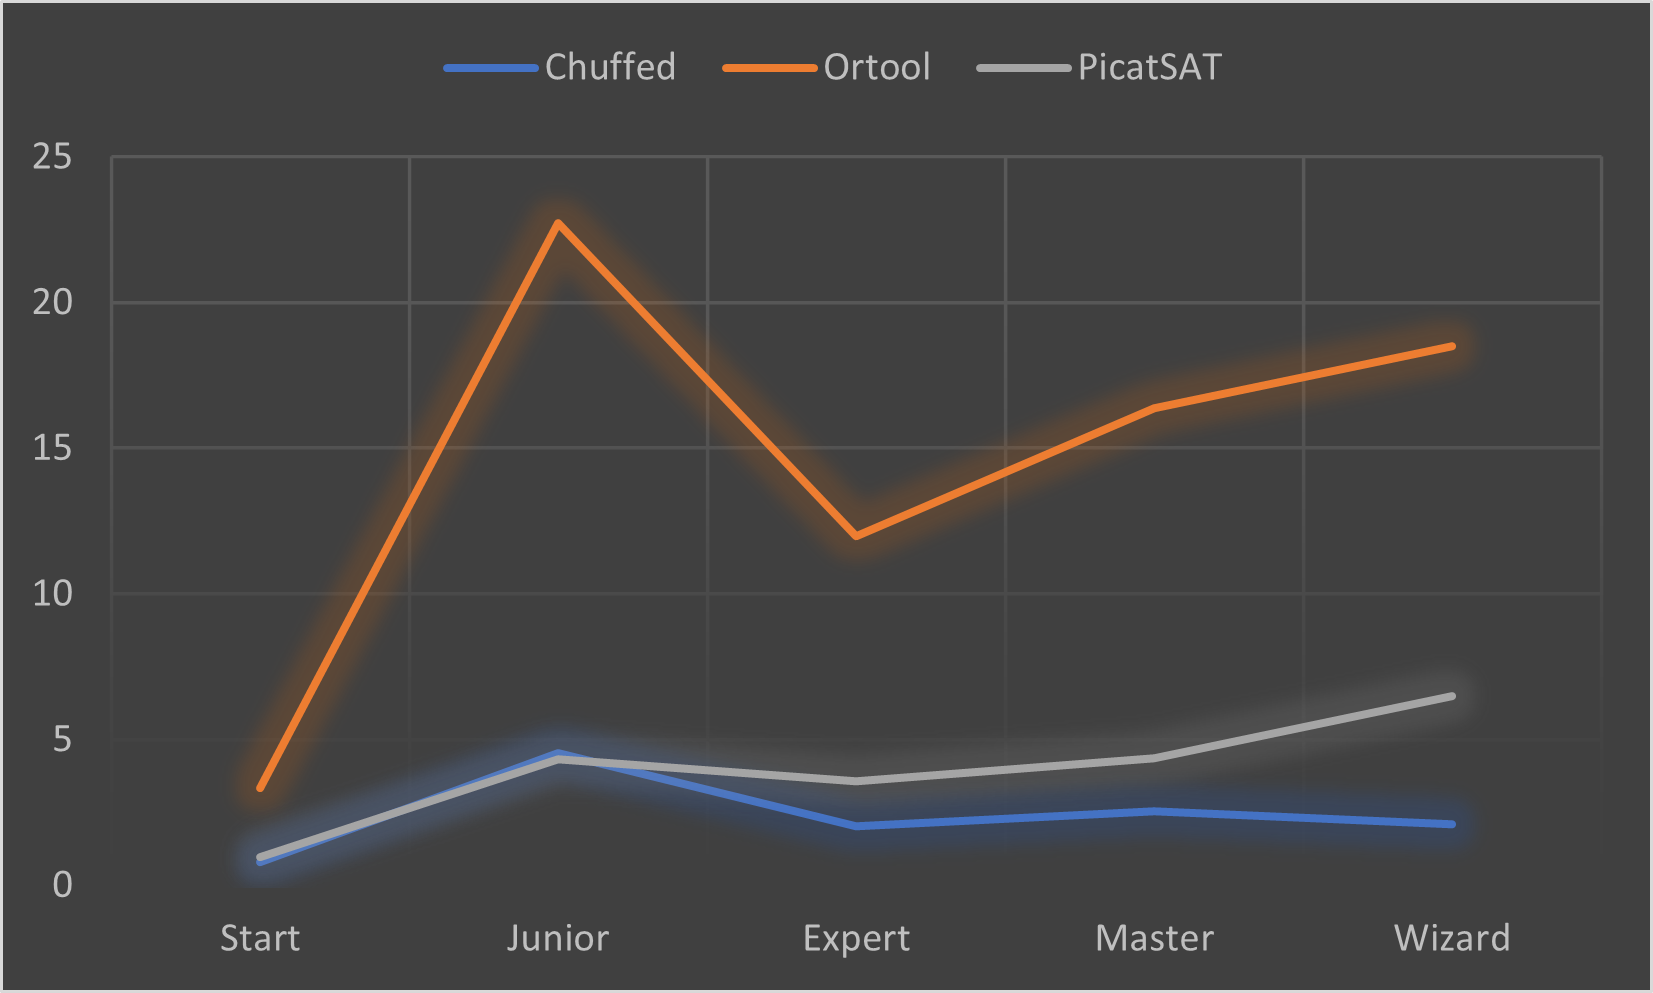
\includegraphics[width=\textwidth]{figs/Three comparison.png}
\caption{Average execution time for Chuffed, PicatSAT and OR-Tools}
\label{fig:3comparison}
\end{subfigure}
\caption{Comparisons between Chuffed, PicatSAT and OR-Tools}
\label{fig:3comparisonsssss}
\end{figure}
Therefore, it is worthy to compare the three solvers more closely. Specifically, according to Figure~\ref{fig:3solvers1}, most of the execution time of Chuffed and PicatSAT are close, and they are usually better than OR-Tools.
Furthermore, Figure~\ref{fig:3comparison} indicates that Chuffed spends less time than PicatSAT except in the "junior" difficulty.
\\In short, although all of Chuffed, PicatSAT and OR-Tools can get the result for each problem in 30 minutes, the solver Chuffed possesses the best performance in IQ Twist.
\subsection{Zig Zag Puzzler Results}
\label{sec:Zig Zag Puzzlerresult}
In the Zig Zag Puzzler booklet, there is a total of 80 problems, 40 of them belong to playing mode1, and the other 40 belong to playing mode2. For each playing mode, every 8 problems make up a difficulty level. 
\subsubsection{Playing Mode1}
Firstly, for each solver, we can calculate the coverage rates by Equation~\ref{equation:coverage}.
\begin{table}[htbp]
\centering
\caption{Overall solved problems of each solver for playing mode1 (a total of 40 problems)}
\label{tab:solvedproblem1}
\begin{tabular}{|l|l|l|l|l|l|l|l|l|}
\hline
Choco & Chuffed & Coinbc& Gurobi & Izplus&Jacop& OR-Tools& PicatSAT&Yuck \\
\hline
40   &40      & 20    & 35    &29     &33   &40    &40      &20\\
\hline
\end{tabular}
\end{table}
According to the data in Table~\ref{tab:solvedproblem1}, Figure~\ref{fig:mode1eva2} indicates that there are 4 solvers that keep 100 percent coverage rates.
\begin{figure}[H]
     \centering
    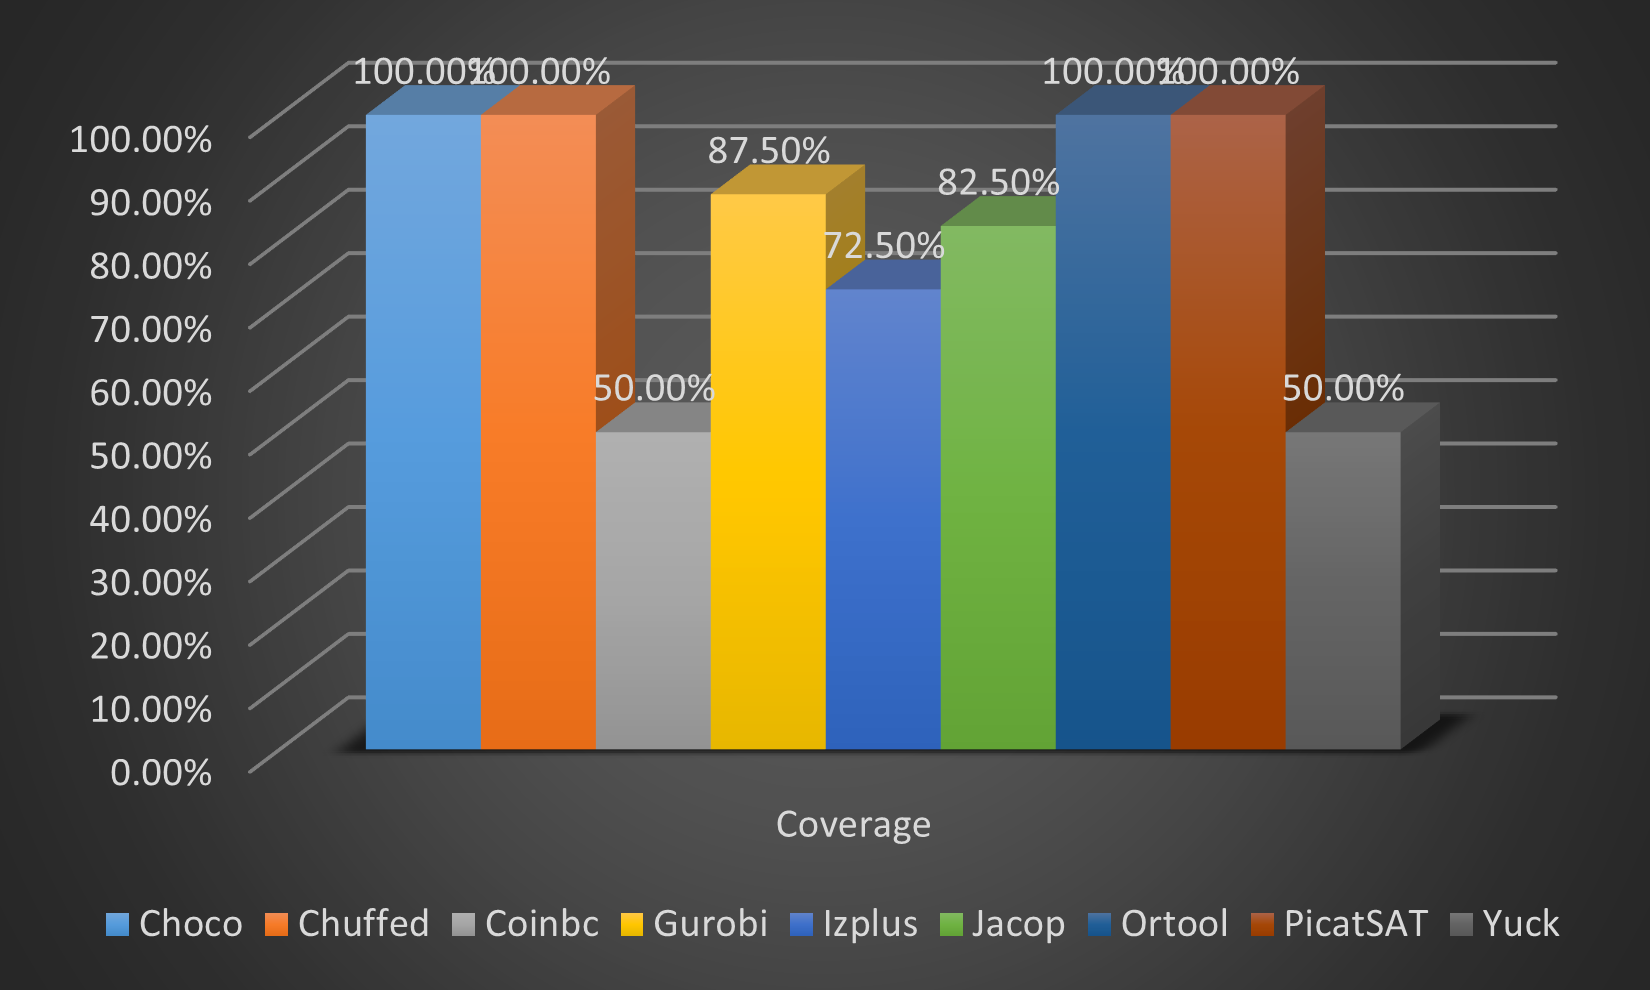
\includegraphics[width=0.8\textwidth]{figs/mode1coverage.png}
    \caption{Overall coverage rates of each solver for playing mode1}
    \label{fig:mode1eva2}
\end{figure}
In addition, on account of Table~\ref{tab:solvedproblemforeach difficulty1}, Figure~\ref{fig:mode1eva4} reveals that except for the four solvers that always keep 100 percent coverage rates in all difficulties, the other five solvers' separated coverage rates are decreased as the difficulties increase.
\begin{table}[H]
\centering
\caption{Solved problems for each difficulty in playing mode1 (a total of 8 problems for each difficulty)}
\label{tab:solvedproblemforeach difficulty1}
\begin{tabular}{|l|l|l|l|l|l|}
\hline
	    &Start	&Junior	&Expert	&Master	&Wizard\\
\hline
Choco	&8	&8	&8	&8	&8\\
\hline
Chuffed	&8	&8	&8	&8	&8\\
\hline
Coinbc	&8	&8	&4	&0	&0\\
\hline
Gurobi	&8	&8	&8	&8	&3\\
\hline
Izplus	&8	&8	&8	&4	&1\\
\hline
Jacop	&8	&8	&8	&5	&4\\
\hline
OR-Tools	&8	&8	&8	&8	&8\\
\hline
PicatSAT	&8	&8	&8	&8	&8\\
\hline
Yuck	&8	&8	&4	&0	&0\\
\hline
\end{tabular}
\end{table}
That is quite reasonable because of the higher difficulty the fewer placed pieces in this playing mode. The fewer placed pieces means the more search nodes, which causes the solver need more time to find the solution.
\begin{figure}[H]
    \centering
    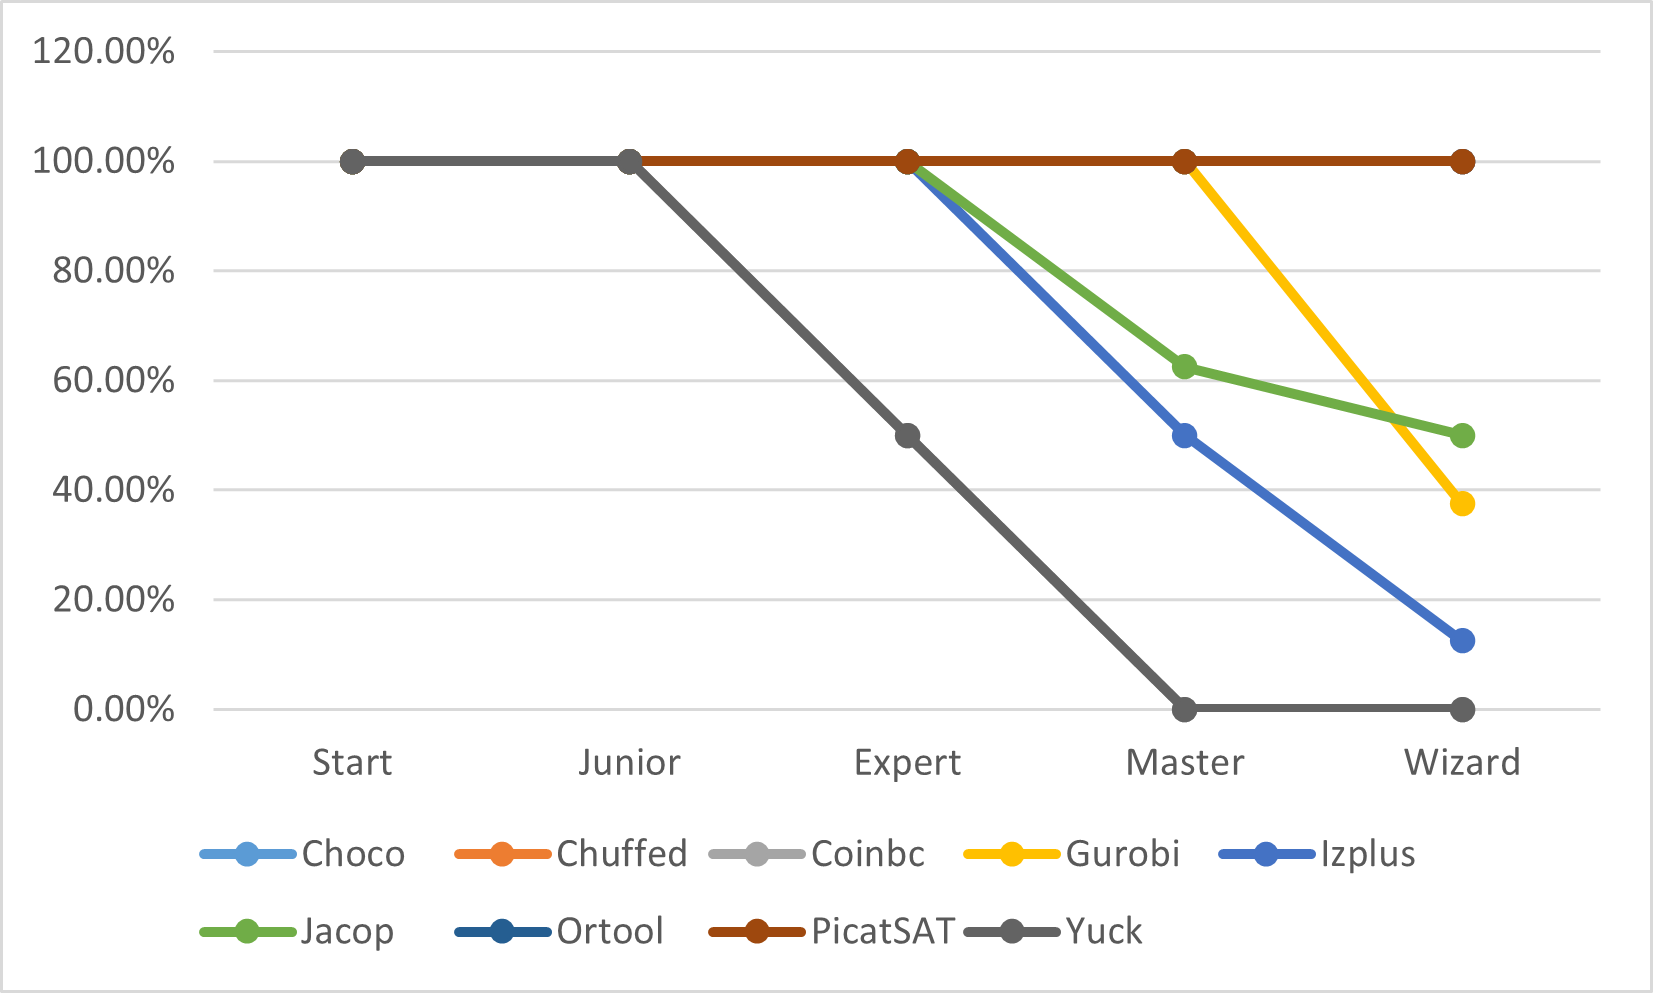
\includegraphics[width=0.8\textwidth]{figs/mode1seperatedcoverage.png}
    \caption{Coverage rates of each difficulty for playing mode1}
    \label{fig:mode1eva4}
\end{figure}
For execution time, Figure~\ref{fig:mode1time1} illustrates that except Choco which spends a lot of time on some problems in  "wizard" difficulty, the other 3 solvers that contain 100 percent overall coverage rates only need a very short time to solve each problem. 
\begin{figure}[htbp]
\centering
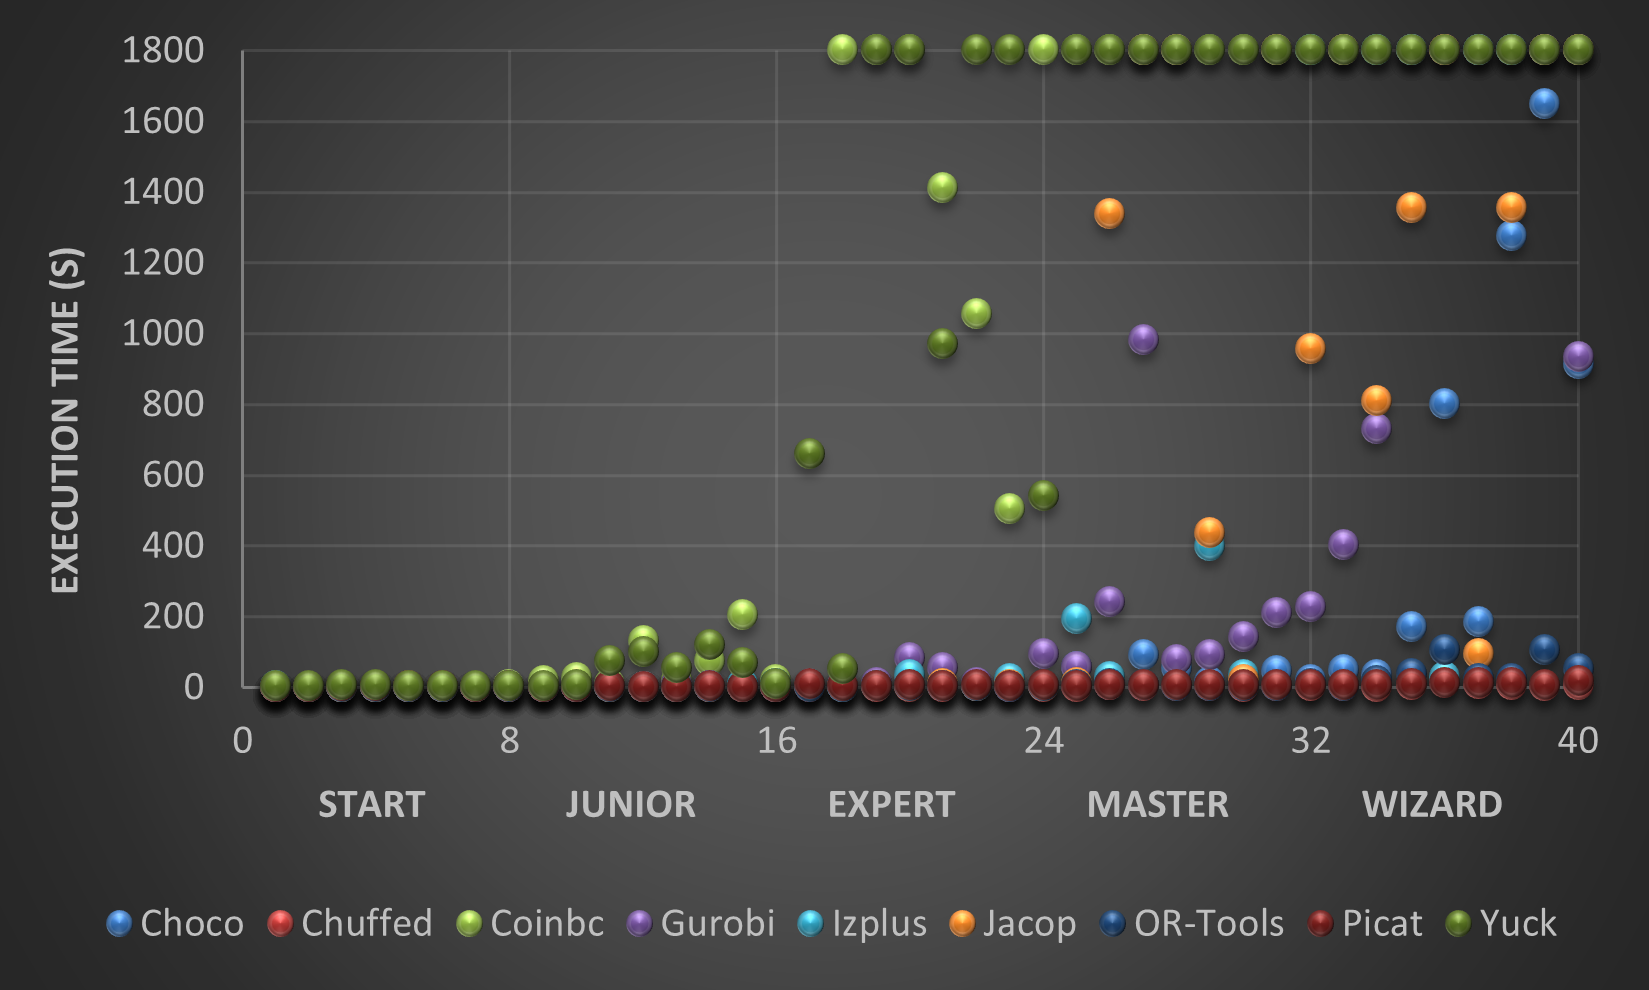
\includegraphics[width=0.8\textwidth]{figs/time1all.png}
\caption{All execution time of all solvers for playing mode1}
\label{fig:mode1time1}
\end{figure}
Moreover, Figure~\ref{fig:time1three} reveals that for the problems in "wizard" difficulty, OR-Tools and PicatSAT spend more time on more problems compared with Chuffed. Accordingly, in Figure~\ref{fig:time1threeslope}, although the start point is very close, the growth rate of slopes for Chuffed is much slower than OR-Tools and PicatSAT. Meanwhile, Figure~\ref{fig:mode1time1} reveals an obvious positive correlation between the execution time of different solvers and the difficulties due to the increased number of search nodes. Therefore, Chuffed has the optimal performance in execution time because of the lowest growth rate of slopes. 
\begin{figure}[htbp]
    \centering
    \begin{subfigure}[b]{0.48\textwidth}
     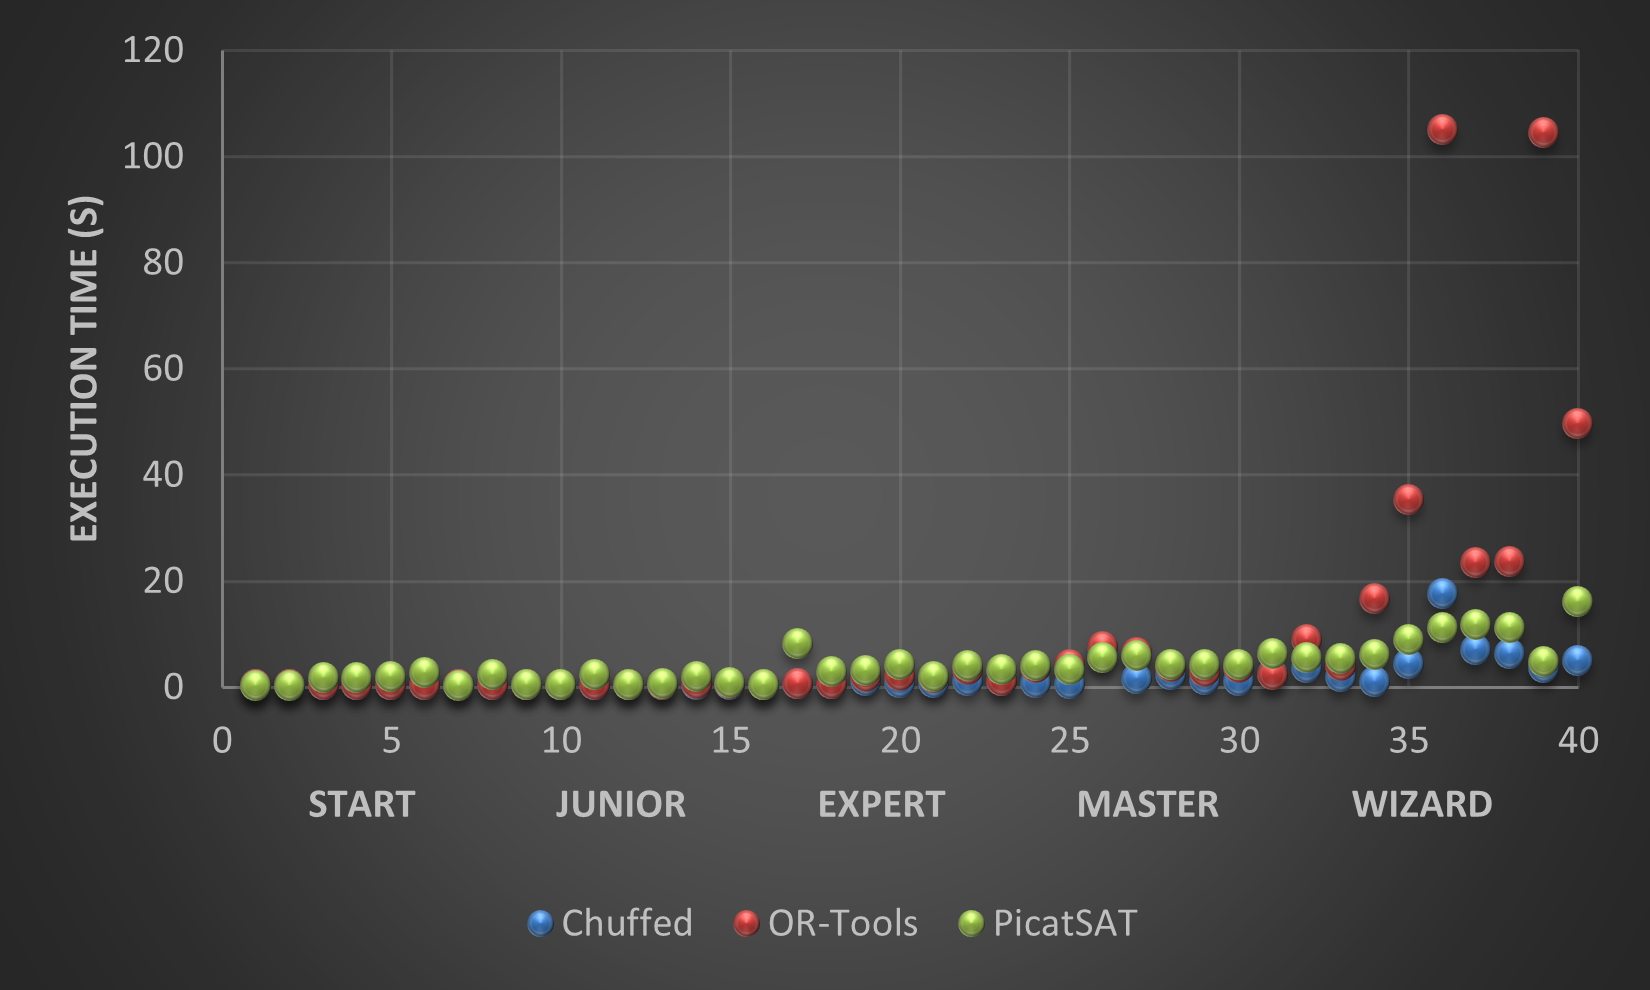
\includegraphics[width=\textwidth]{figs/time1three.png}
    \caption{Execution time for Chuffed, PicatSAT and OR-Tools}
    \label{fig:time1three}
    \end{subfigure}
    \begin{subfigure}[b]{0.48\textwidth}
     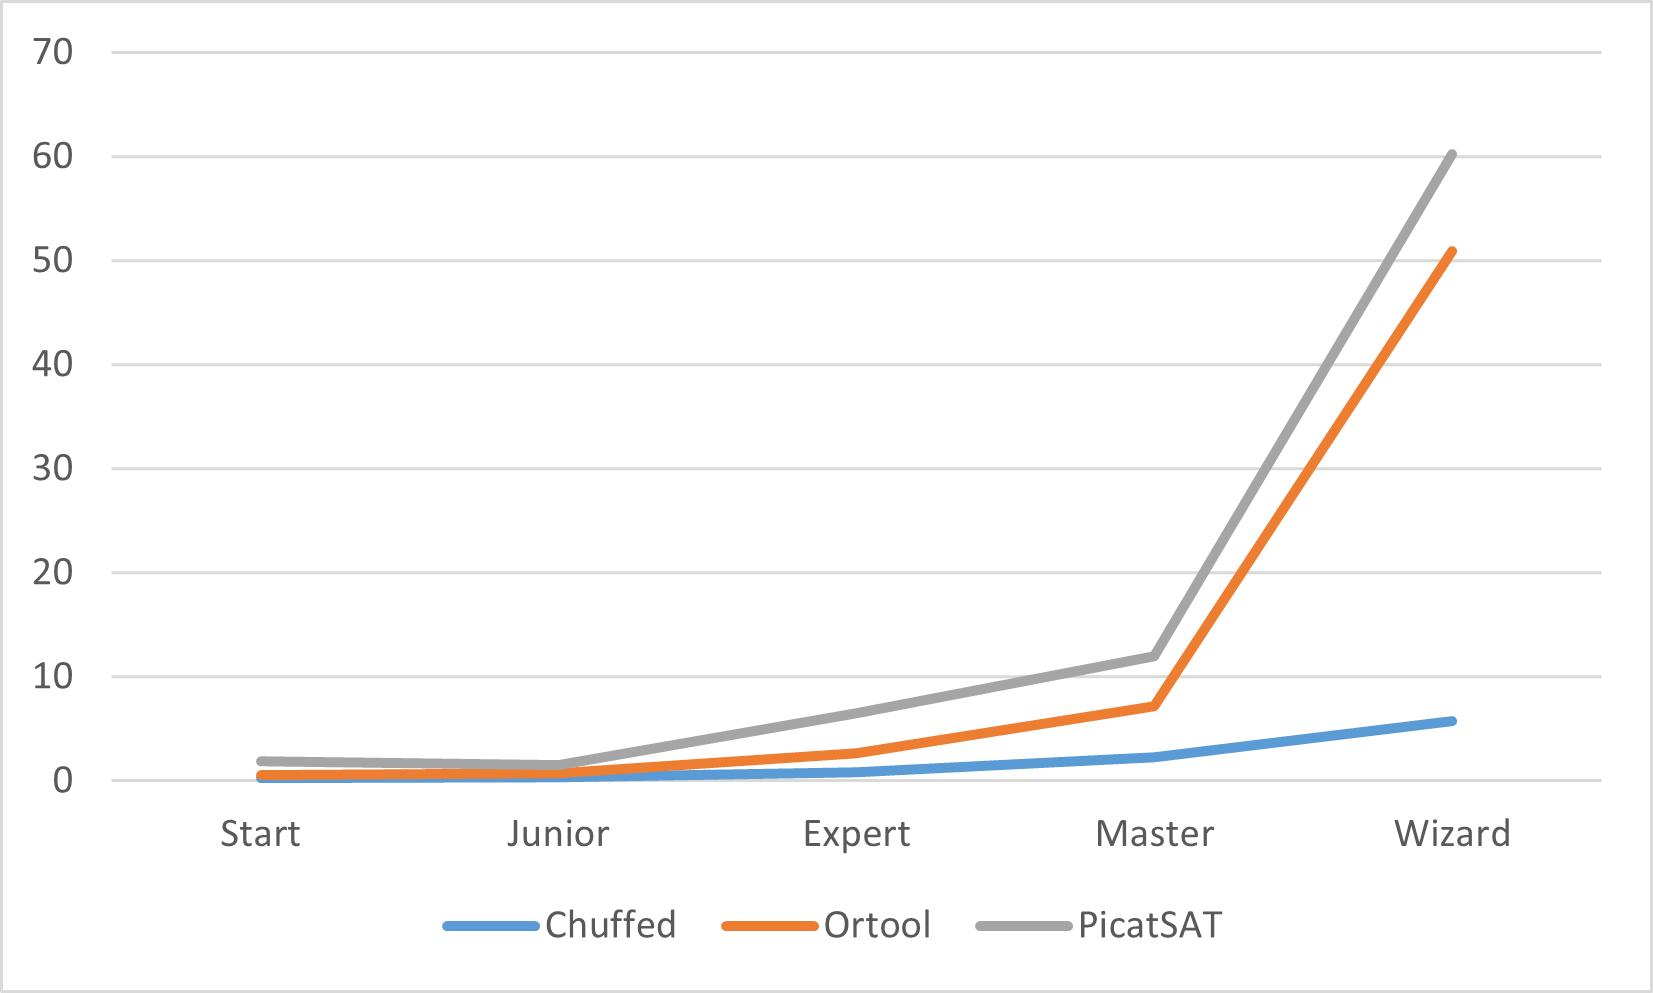
\includegraphics[width=\textwidth]{figs/mode1solverscomparison.png}
    \caption{Average execution time for Chuffed, PicatSAT and OR-Tools}
    \label{fig:time1threeslope}
    \end{subfigure}
    \caption{Comparisons between Chuffed, PicatSAT and OR-Tools for playing mode1}
\end{figure}
Overall, combined coverage rates and execution time, Chuffed possesses the best performance in Zig Zag Puzzler playing mode1.
\subsubsection{Playing Mode2}
\begin{table}[H]
\centering
\caption{Overall solved problems of each solver for playing mode2 (a total of 40 problems)}
\label{tab:solvedproblem2}
\begin{tabular}{|l|l|l|l|l|l|l|l|l|}
\hline
Choco & Chuffed & Coinbc& Gurobi & Izplus&Jacop& OR-Tools& PicatSAT&Yuck \\
\hline
37   &40      & 12    & 34    &35     &32   &40    &40      &22\\
\hline
\end{tabular}
\end{table}
Based on Table~\ref{tab:solvedproblem2}, as is shown in Figure~\ref{fig:mode2eva2}, the result of coverage rates is quite similar to the result of coverage rates in playing mode 1 because the rule of playing mode2 is quite similar to playing mode1. Both of them set fewer pieces as difficulty increases. In addition, they use the same pieces.
\begin{figure}[H]
     \centering
    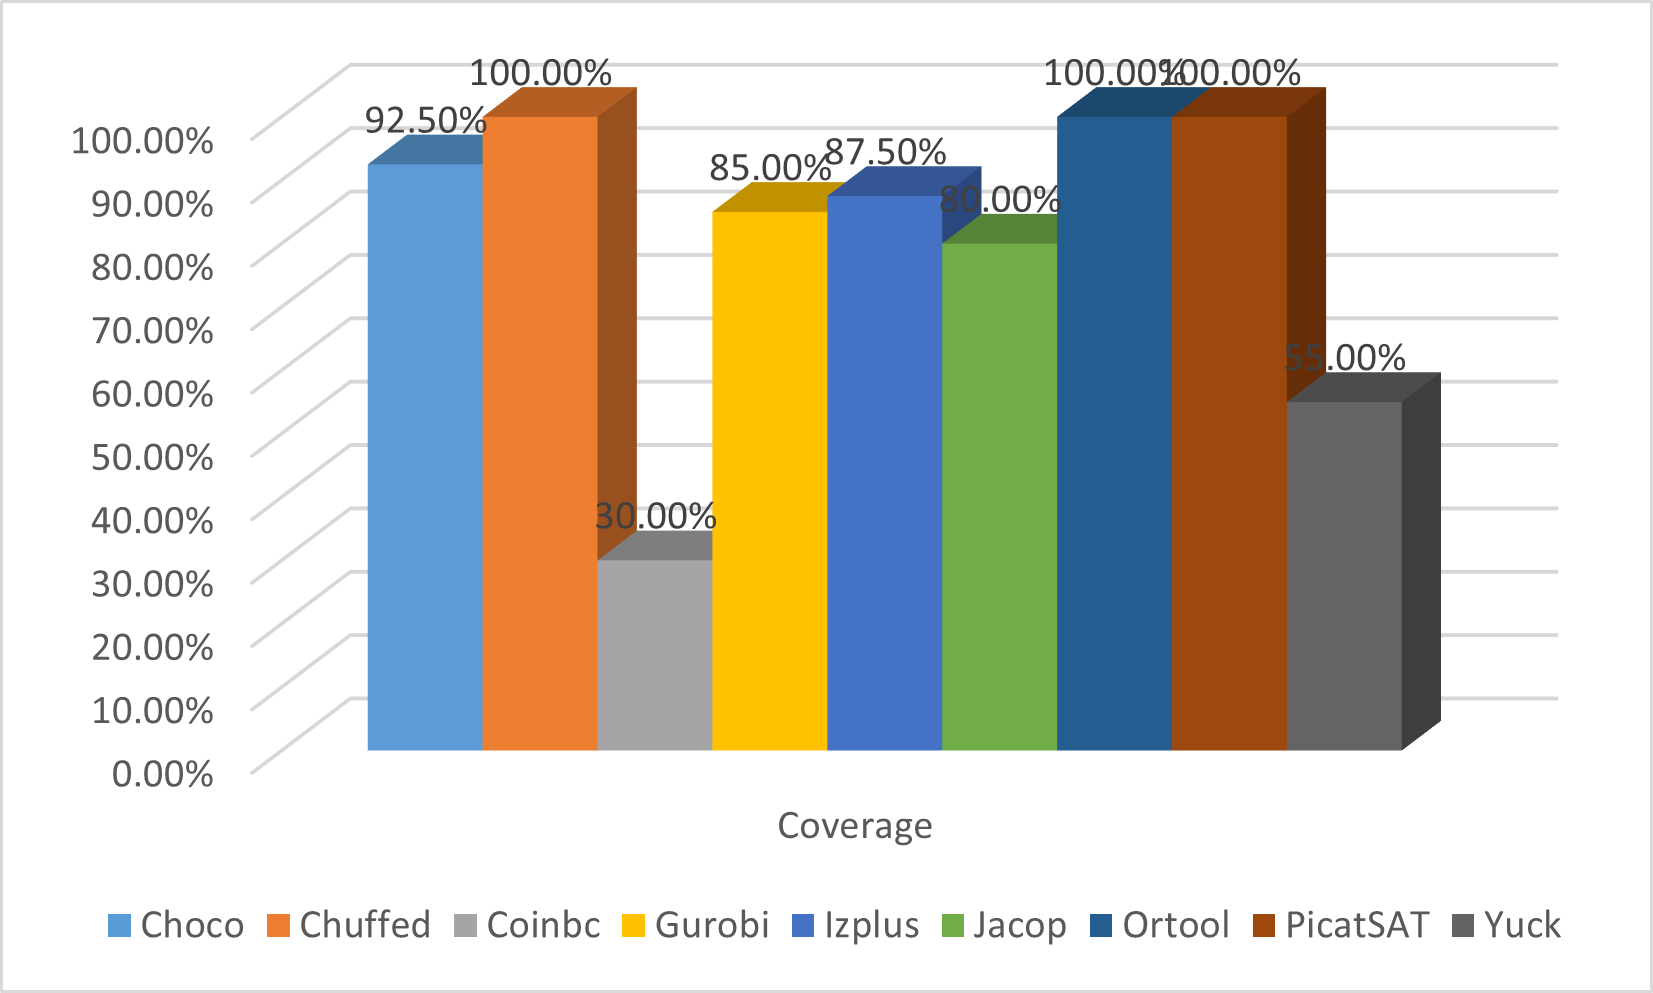
\includegraphics[width=0.8\textwidth]{figs/mode2coverage.png}
    \caption{Overall coverage rates of each solver for playing mode2}
    \label{fig:mode2eva2}
\end{figure}
Again, Chuffed, PicatSAT and OR-Tools solve each problem in 30 minutes. 
\begin{table}[H]
\centering
\caption{Solved problems of each difficulty for playing mode2 (a total of 8 problems for each difficulty)}
\label{tab:solvedproblemforeach difficulty2}
\begin{tabular}{|l|l|l|l|l|l|}
\hline
	    &Start	&Junior	&Expert	&Master	&Wizard\\
\hline
Choco	&8	&8	&8	&8	&5\\
\hline
Chuffed	&8	&8	&8	&8	&8\\
\hline
Coinbc	&7	&5	&0	&0	&0\\
\hline
Gurobi	&8	&8	&8	&7	&3\\
\hline
Izplus	&8	&8	&8	&7	&4\\
\hline
Jacop	&8	&8	&8	&7	&1\\
\hline
OR-Tools	&8	&8	&8	&8	&8\\
\hline
PicatSAT	&8	&8	&8	&8	&8\\
\hline
Yuck	&8	&8	&4	&2	&0\\
\hline
\end{tabular}
\end{table}
Meanwhile, according to the data in Table~\ref{tab:solvedproblemforeach difficulty2}, Figure~\ref{fig:mode2eva4} indicates that the other 6 solvers' separated coverage rates are decreased as the difficulties increase, which is also very similar to playing mode1.
 \begin{figure}[H]
   \centering
    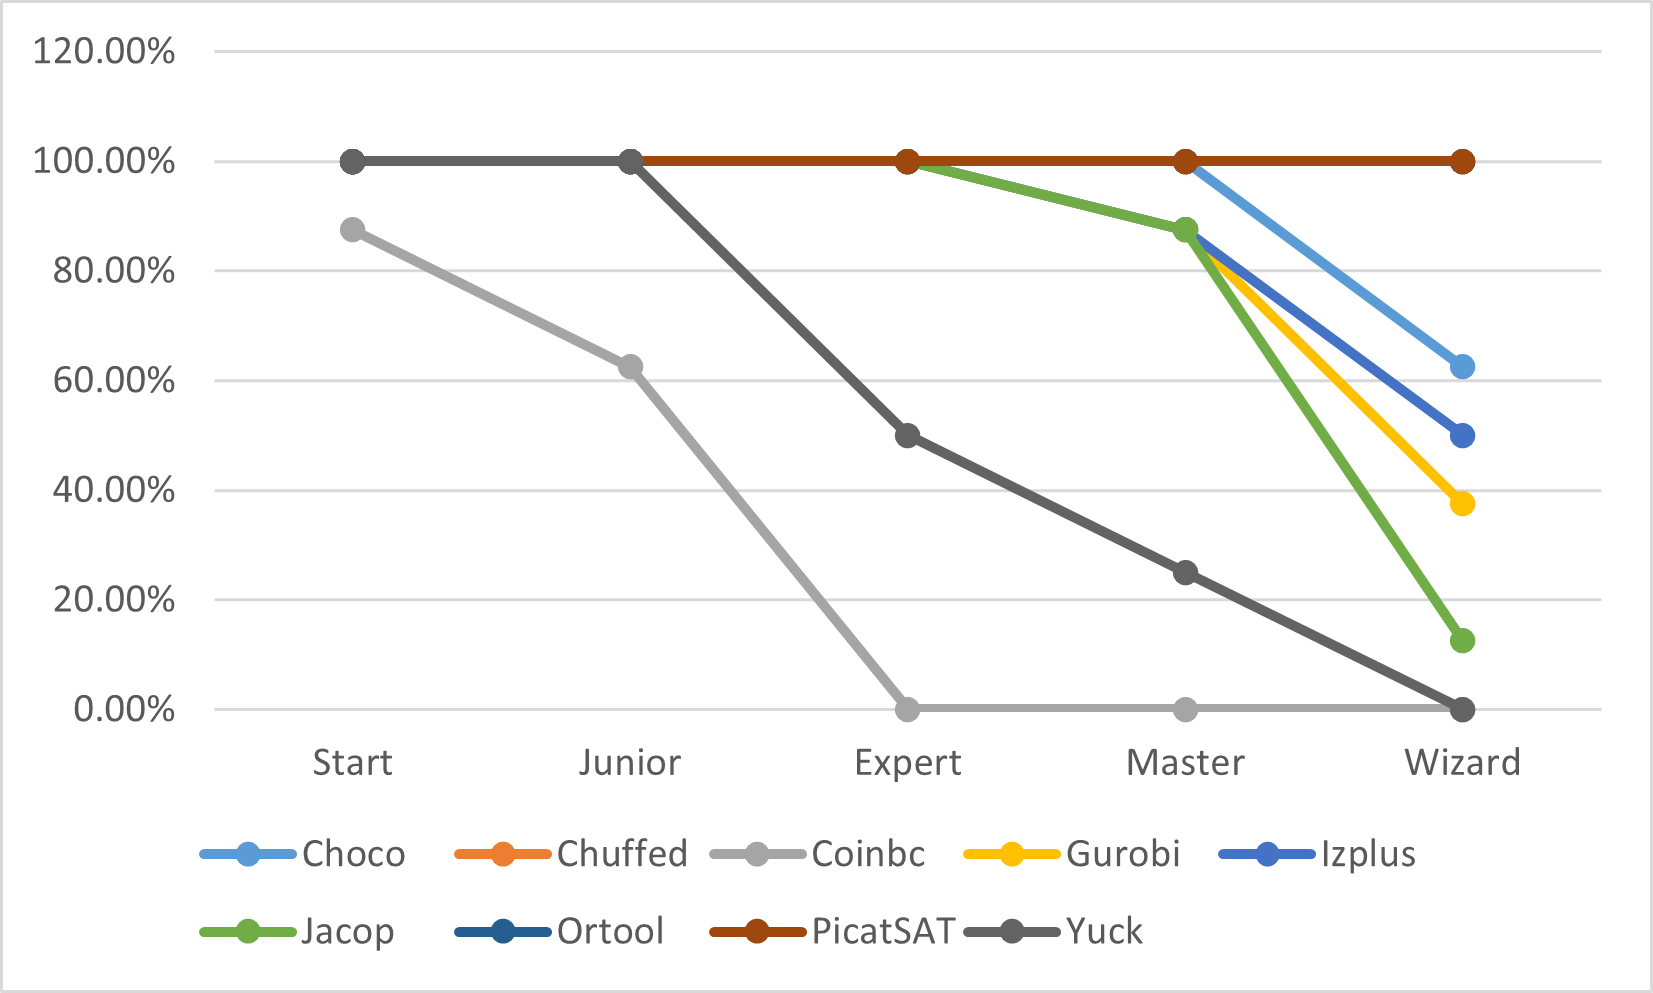
\includegraphics[width=0.8\textwidth]{figs/mode2seperatedcoverage.png}
    \caption{Coverage rates of each difficulty in playing mode2}
    \label{fig:mode2eva4}
\end{figure}
For the execution time, as is shown in Figure~\ref{fig:mode2time2}, almost all the solvers' execution time has a positive correlation with the difficulties. Again, Chuffed, PicatSAT and OR-Tools spend less time to solve most problems. 
\begin{figure}[H]
    \centering
    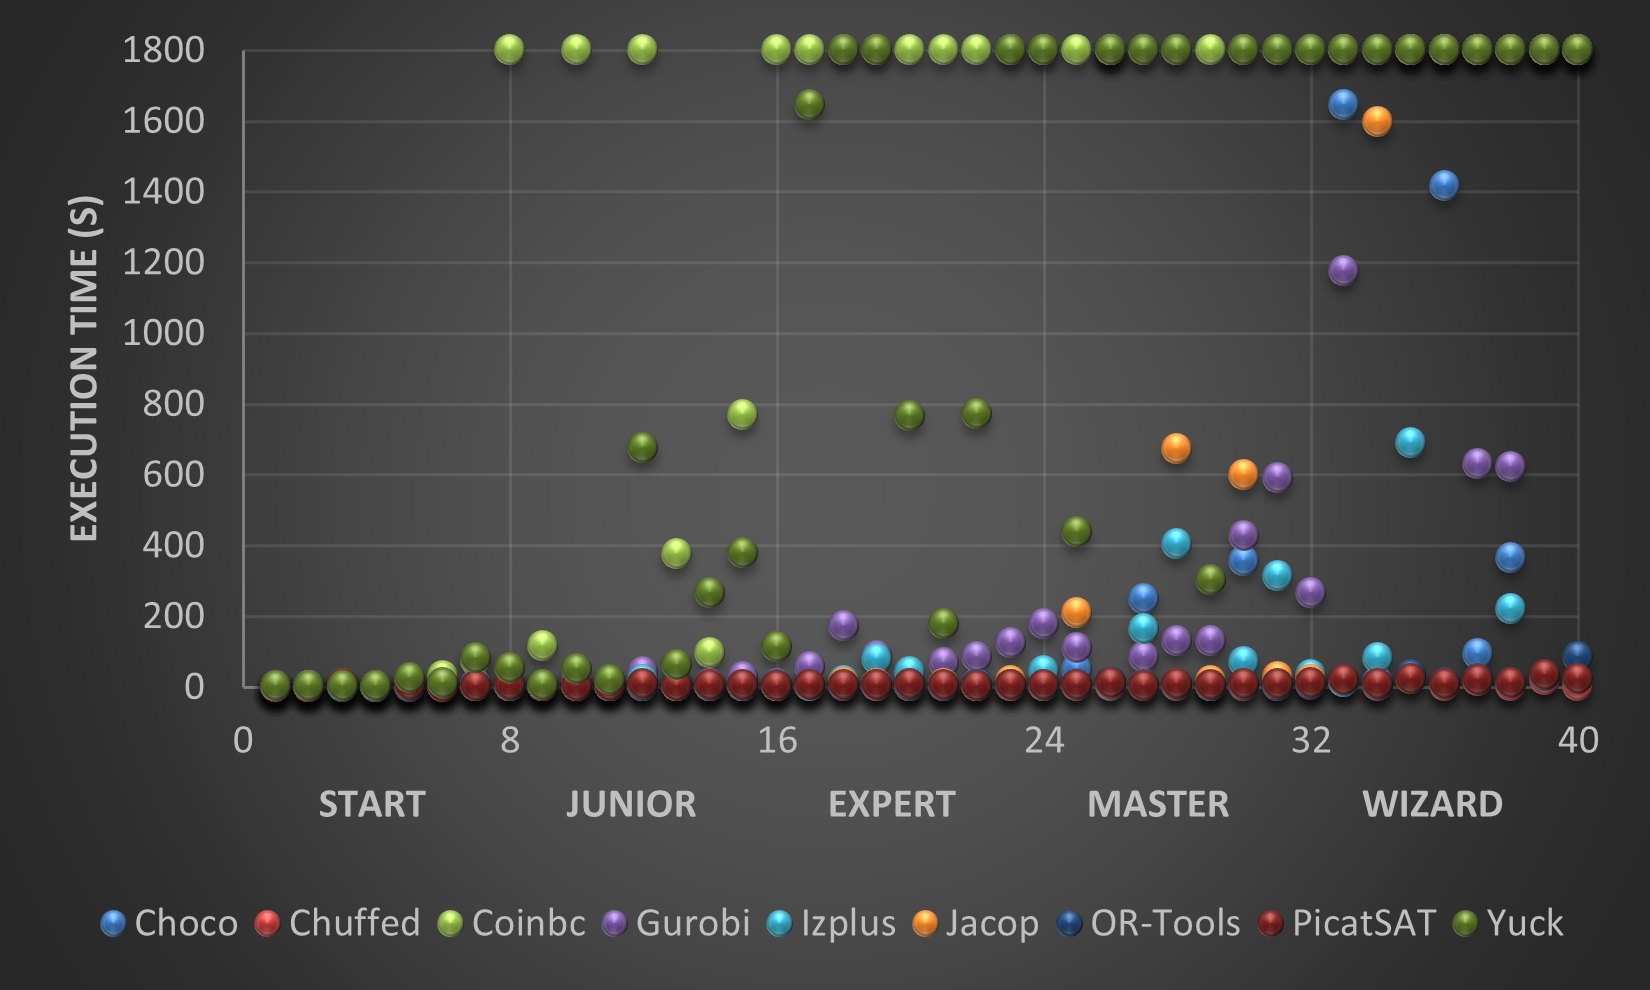
\includegraphics[width=0.8\textwidth]{figs/time2all.png}
    \caption{All execution time of all solvers for playing mode2}
    \label{fig:mode2time2}
\end{figure}
Similarly, on account of Figure~\ref{fig:comparisonlast}, Chuffed achieves optimal performance. 
\begin{figure}[H]
\begin{subfigure}[b]{0.48\textwidth}
  \centering
    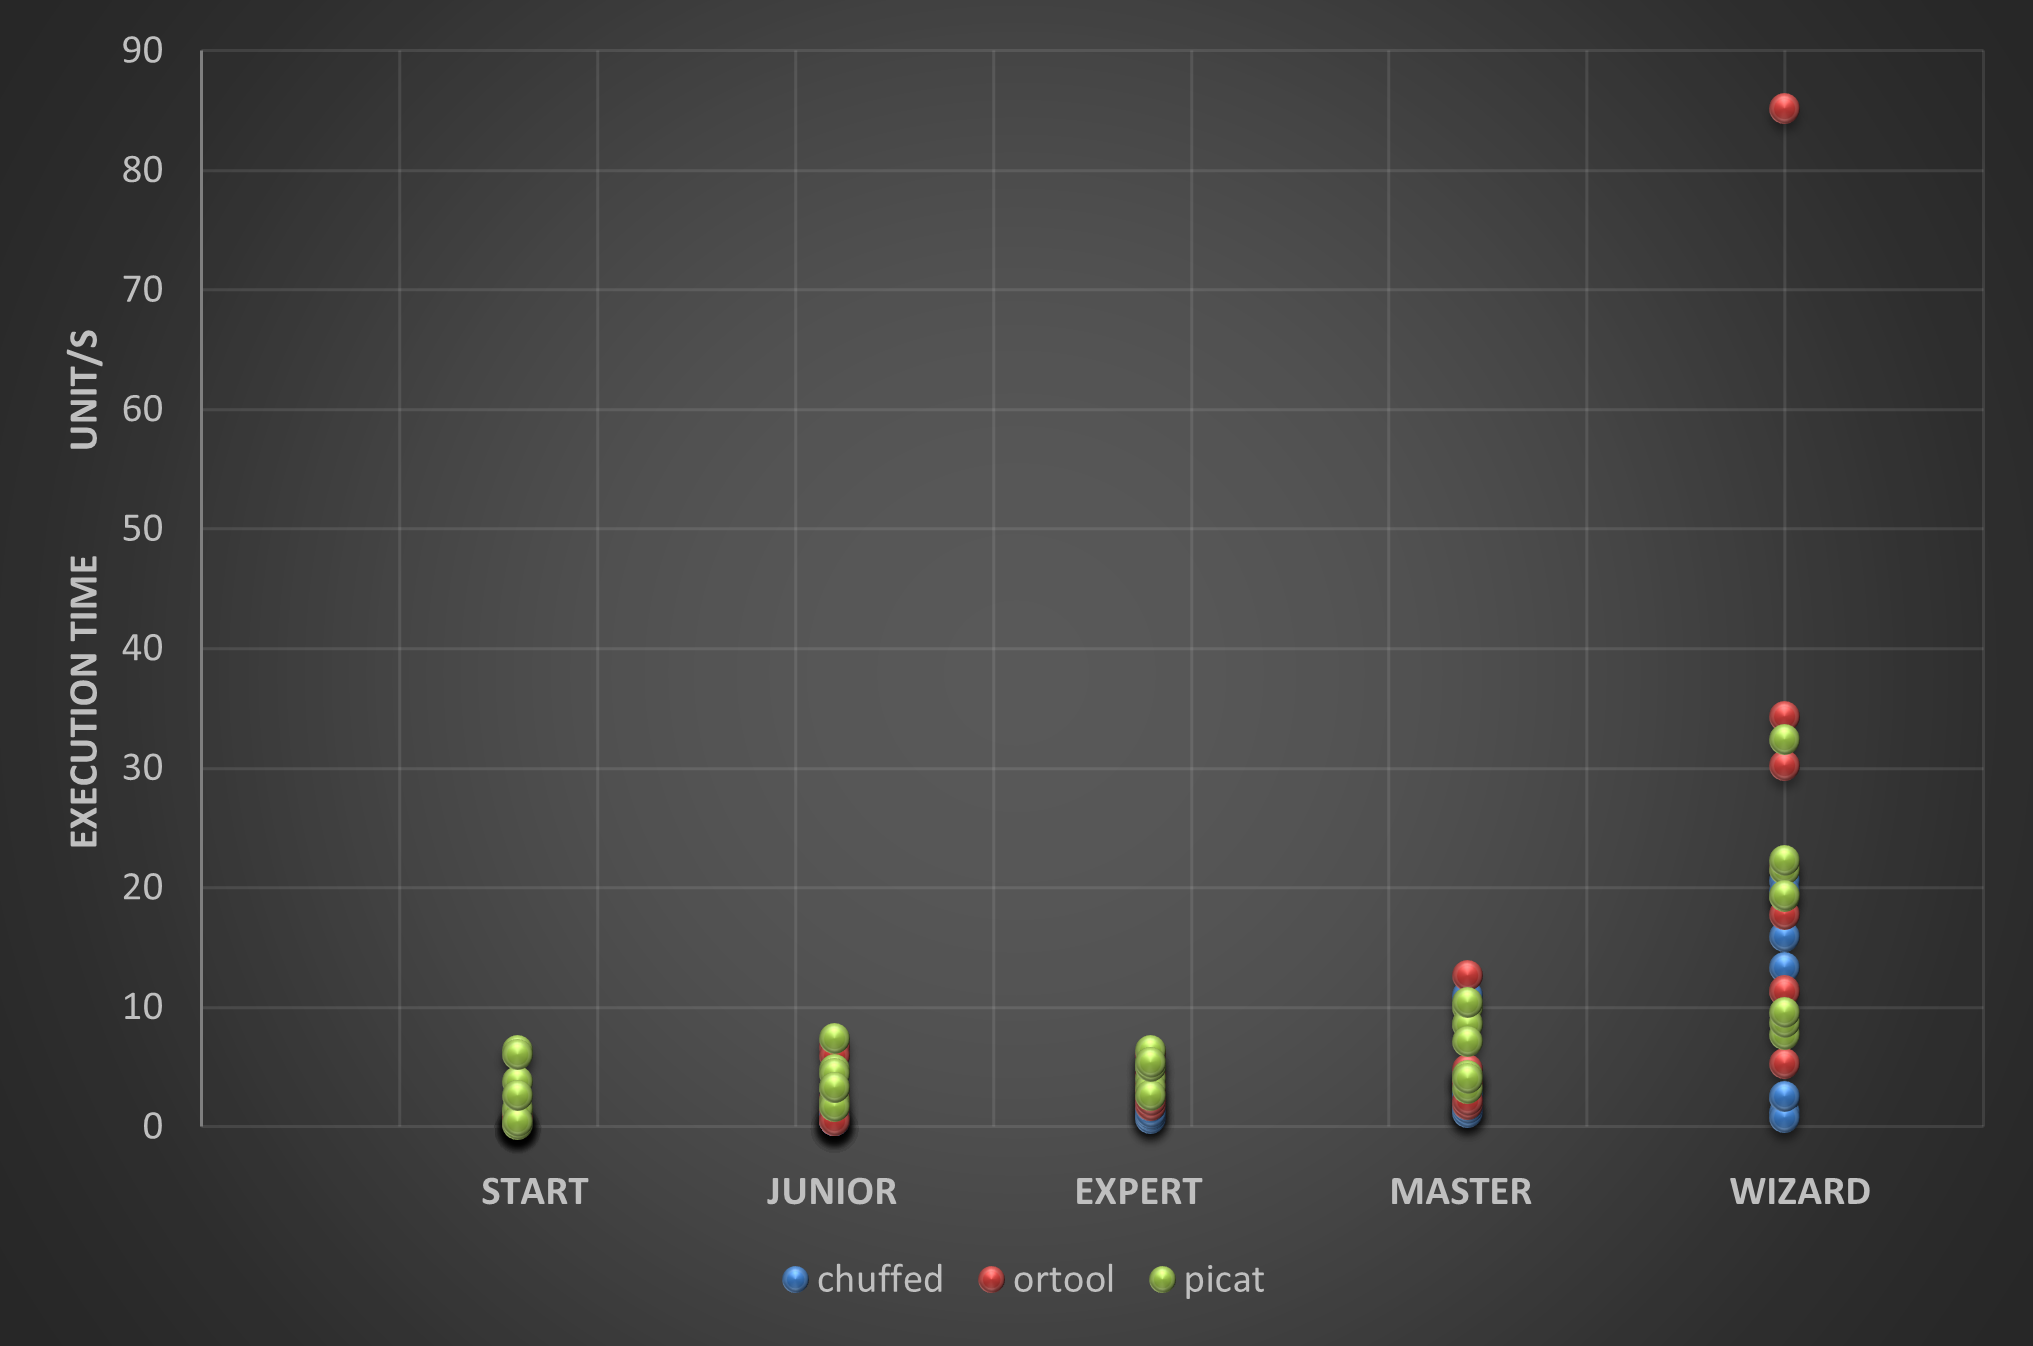
\includegraphics[width=\textwidth]{figs/time2three.png}
    \caption{Execution time for Chuffed, PicatSAT and OR-Tools}
    \label{fig:compare}
\end{subfigure}
\begin{subfigure}[b]{0.48\textwidth}
 \centering
    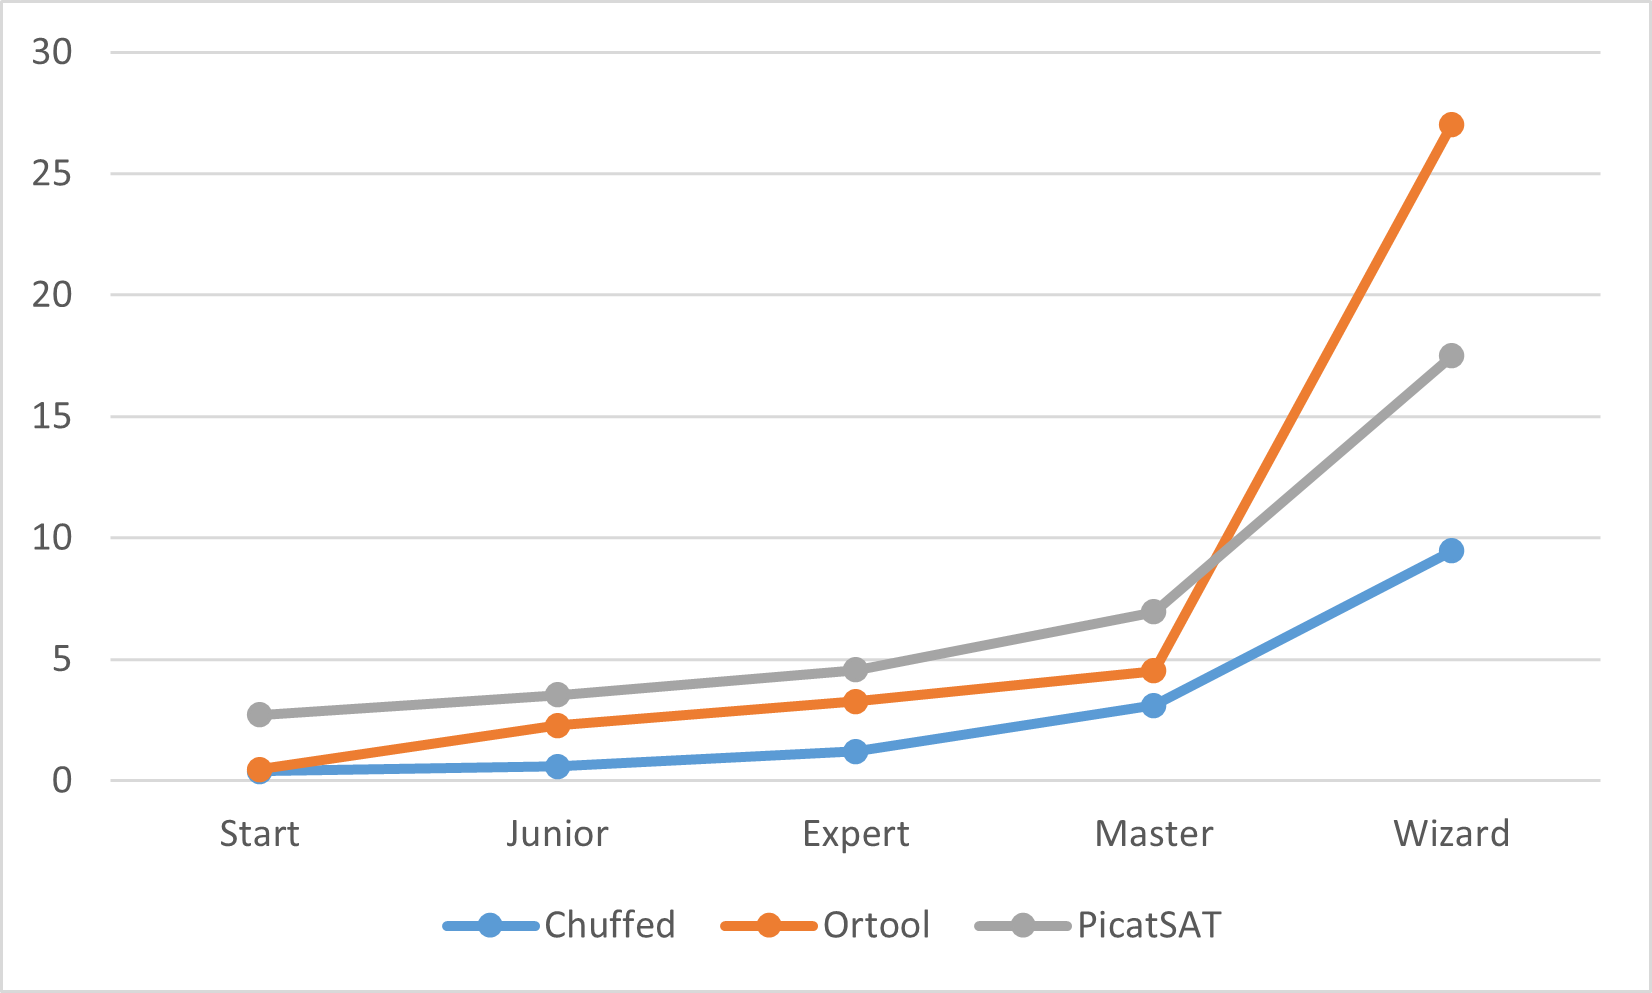
\includegraphics[width=\textwidth]{figs/Threecomparison2.png}
    \caption{Average execution time for Chuffed, PicatSAT and OR-Tools}
    \label{fig:compare}
\end{subfigure}
\caption{Comparisons between Chuffed, PicatSAT and OR-Tools for playing mode2}
\label{fig:comparisonlast}
\end{figure}
\subsection{Summary}
\label{sec:Summary}
The different difficulty settings in IQ Twist and Zig Zag Puzzler cause the different relationships between solvers' performance and difficulty in each game. However, for Zig Zag Puzzler, because both playing modes set fewer pieces as the increase of difficulties, the relationships between solvers' performance and the games' difficulty level are very similar. In addition, for all the problems in both IQ Twist and Zig Zag Puzzler, Chuffed, PicatSAT and OR-Tools can solve each of them in 30 minutes. Meanwhile, their performances are more stable and the average execution time for all problems is only a few seconds. To sum up, compared with other solvers, Chuffed, PicatSAT and OR-Tools have obvious advantages in such problems, moreover, Chuffed cost the shortest time in most problems. 
 